%=======================+==============================
%============    Summary   =============
%======================================================

\section{Summary and outlook\label{sec:summary} }
We have presented the design, construction, and performance, of the beamline and detector of the \gx{} experiment in Hall D at Jefferson Lab during its first phase of operation. The experiment operated routinely at an incident photon flux of $2\times 10^{7}$ photons/s in the coherent peak with an open trigger, taking data at 40 kHz, and recording 600 MB/s to tape with live time $>$95\%. During this period the experiment accumulated  121.4 pb$^{-1}$ in the coherent peak and 319.4 pb$^{-1}$ total for $E_\gamma>$8.1 GeV. Data were collected in two sets of orthogonal linear polarizations of the incident photons, with $\sim$23\% of the data in each of the four orientations. The remaining $\sim$11\% was collected with unpolarized photons. Approximately 270 billion triggers were accumulated during this period, as shown in Fig.\,\ref{fig:plot_rcdb3_phaseI}.  

\begin{figure}[tbh]\centering
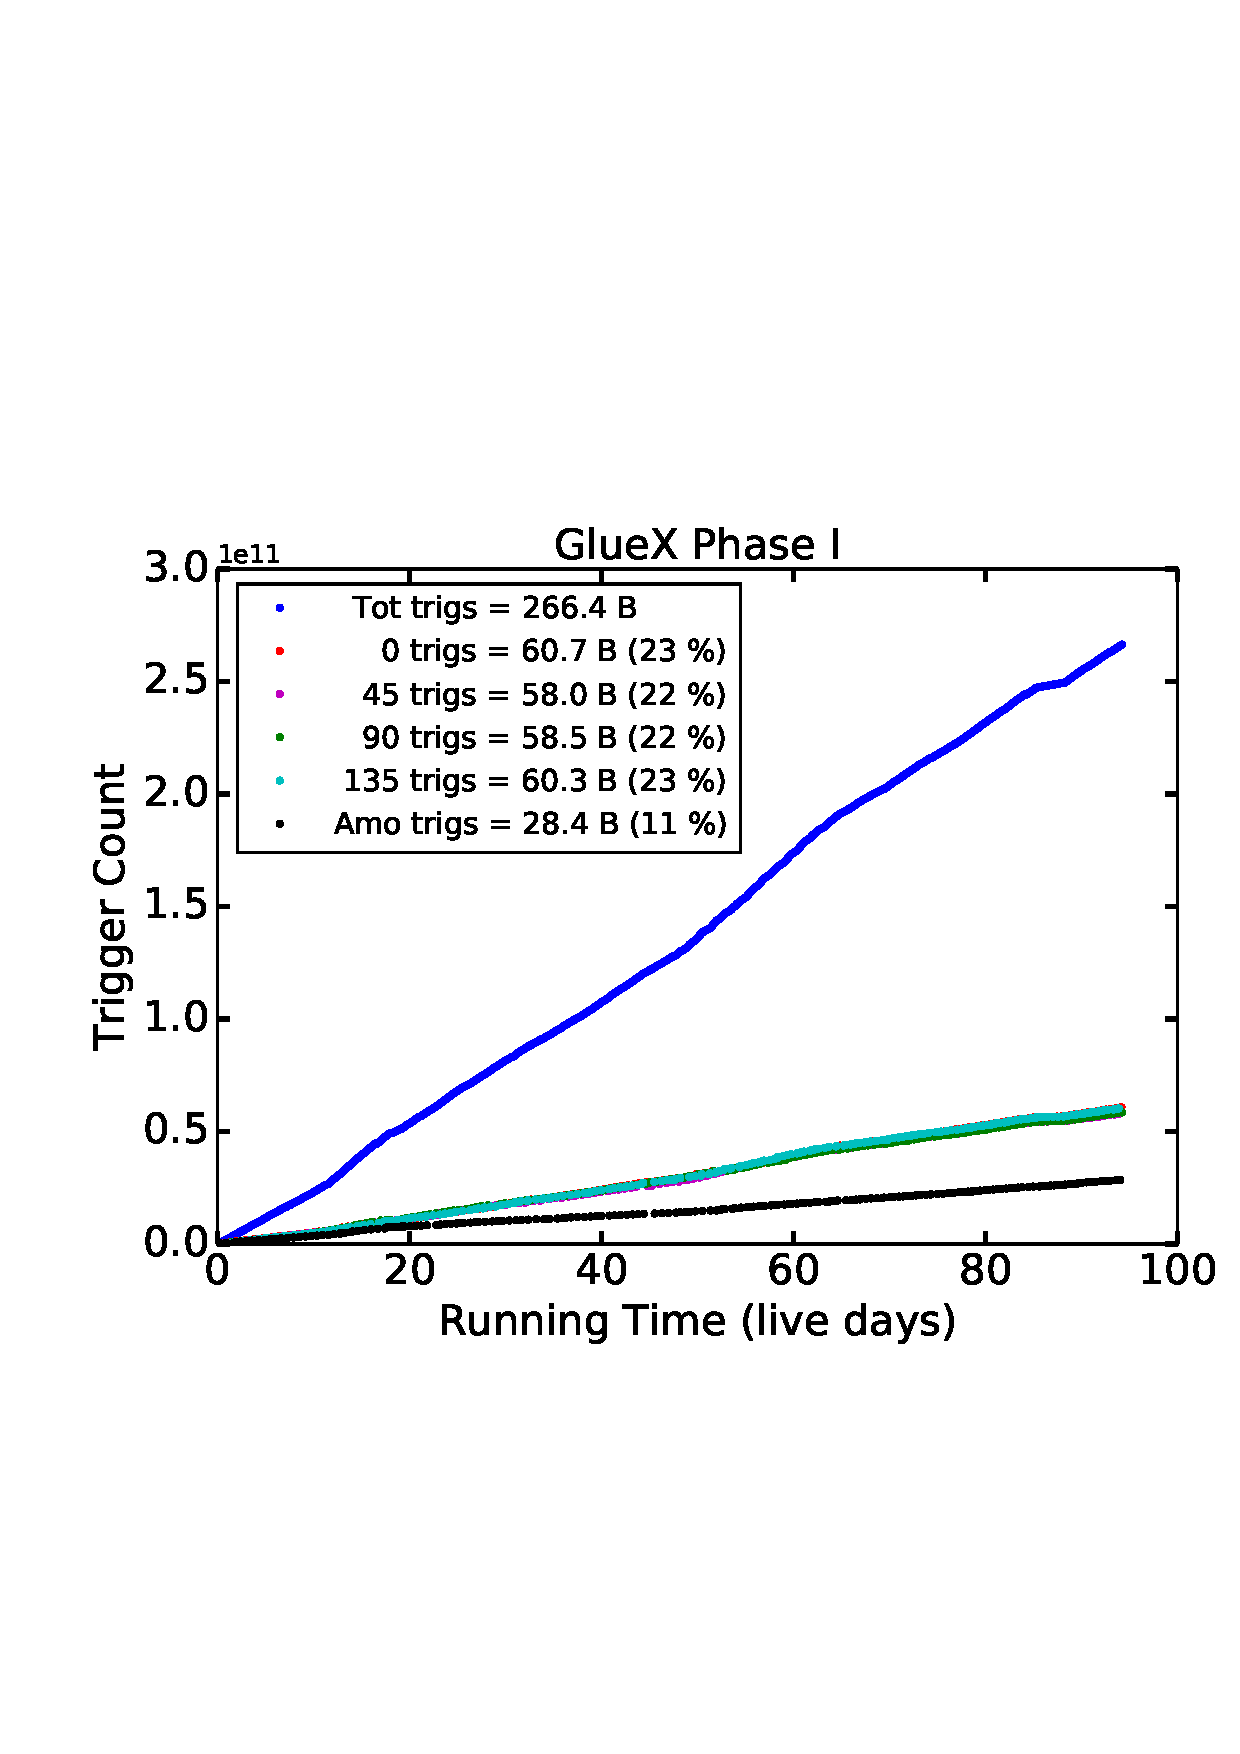
\includegraphics[width=0.48\textwidth]{figures/plot_rcdb3_phaseI.pdf}
\caption{\label{fig:plot_rcdb3_phaseI} 
Plot of integrated number of triggers versus the number of live days in 2017 and 2018. The triggers of the four diamond configurations fall on top of one another, as we attempted to match the amount of data taken for each configuration. 
(Color online)    
 }   
\end{figure}   

The operational characteristics of the charged and neutral particle detectors, trigger, DAQ, online and offline systems have been verified, and individual components performed as designed. The detector is able to reconstruct exclusive final states, reconstruction efficiencies have been determined, and Monte Carlo simulations compare well with experimental data. The infrastructure is in place to process our high volume of data both on the JLab computing farm as well on other offsite facilities, providing the ability to process the data in a timely fashion.

Future running will include taking data at higher luminosity  and with improved particle identification capability. The \gx~experiment has already implemented the necessary infrastructure to allow the experiment to operate at a flux of $5\times10^{7}$ photons/s in the coherent peak for the upcoming run periods and has added a new DIRC detector\footnote{Four ``bar boxes" from the BaBar DIRC\cite{Aubert:2001tu} detector have been installed and tested.} to extend particle identification of kaons to higher momenta. 

